\subsection{x86}

\subsubsection{MSVC}

Let's compile:

\lstinputlisting[caption=MSVC 2008]{patterns/13_arrays/1_simple/simple_msvc.asm}

\myindex{x86!\Instructions!SHL}

Nothing very special, just two loops: the first is a filling loop and second is a printing loop.
The \TT{shl ecx, 1} instruction is used for value multiplication by 2 in \ECX, more about below~\myref{SHR}.

80 bytes are allocated on the stack for the array, 20 elements of 4 bytes.

\clearpage
Let's try this example in \olly.
\myindex{\olly}

We see how the array gets filled: 

each element is 32-bit word of \Tint type and its value is the index multiplied by 2:

\begin{figure}[H]
\centering
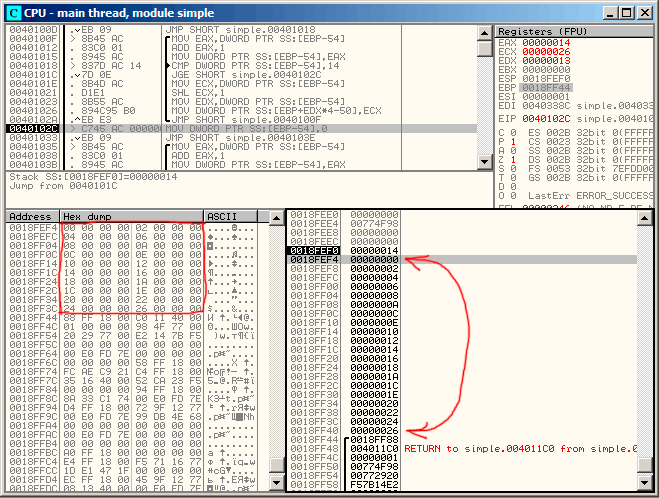
\includegraphics[scale=\FigScale]{patterns/13_arrays/1_simple/olly.png}
\caption{\olly: after array filling}
\label{fig:array_simple_olly}
\end{figure}

Since this array is located in the stack, we can see all its 20 elements there.

\subsubsection{GCC}

Here is what GCC 4.4.1 does:

\lstinputlisting[caption=GCC 4.4.1]{patterns/13_arrays/1_simple/simple_gcc.asm}

By the way, variable $a$ is of type  \IT{int*} 
(the pointer to \Tint{})---you can pass a pointer to an array to another function,
but it's more correct to say that a pointer to the first element of the array is passed
(the addresses of rest of the elements are calculated in an obvious way).

If you index this pointer as \IT{a[idx]}, \IT{idx} is just to be added to the pointer 
and the element placed there (to which calculated pointer is pointing) is to be returned.

An interesting example: a string of characters like 
\IT{\q{string}} is an array of characters and it has a type of \IT{const char[]}.

An index can also be applied to this pointer.

And that is why it is possible to write things like \TT{\q{string}[i]}---this is a correct \CCpp expression!

